% Created 2021-09-11 Sat 08:17
% Intended LaTeX compiler: xelatex
\documentclass[letterpaper]{article}
\usepackage{graphicx}
\usepackage{grffile}
\usepackage{longtable}
\usepackage{wrapfig}
\usepackage{rotating}
\usepackage[normalem]{ulem}
\usepackage{amsmath}
\usepackage{textcomp}
\usepackage{amssymb}
\usepackage{capt-of}
\usepackage{hyperref}
\usepackage[margin=1in]{geometry}
\usepackage{fontspec}
\usepackage{indentfirst}
\setmainfont[ItalicFont = LiberationSans-Italic, BoldFont = LiberationSans-Bold, BoldItalicFont = LiberationSans-BoldItalic]{LiberationSans}
\newfontfamily\NHLight[ItalicFont = LiberationSansNarrow-Italic, BoldFont       = LiberationSansNarrow-Bold, BoldItalicFont = LiberationSansNarrow-BoldItalic]{LiberationSansNarrow}
\newcommand\textrmlf[1]{{\NHLight#1}}
\newcommand\textitlf[1]{{\NHLight\itshape#1}}
\let\textbflf\textrm
\newcommand\textulf[1]{{\NHLight\bfseries#1}}
\newcommand\textuitlf[1]{{\NHLight\bfseries\itshape#1}}
\usepackage{fancyhdr}
\pagestyle{fancy}
\usepackage{titlesec}
\usepackage{titling}
\makeatletter
\lhead{\textbf{\@title}}
\makeatother
\rhead{\textrmlf{Compiled} \today}
\lfoot{\theauthor\ \textbullet \ \textbf{2021-2022}}
\cfoot{}
\rfoot{\textrmlf{Page} \thepage}
\titleformat{\section} {\Large} {\textrmlf{\thesection} {|}} {0.3em} {\textbf}
\titleformat{\subsection} {\large} {\textrmlf{\thesubsection} {|}} {0.2em} {\textbf}
\titleformat{\subsubsection} {\large} {\textrmlf{\thesubsubsection} {|}} {0.1em} {\textbf}
\setlength{\parskip}{0.45em}
\renewcommand\maketitle{}
\author{Houjun Liu}
\date{\today}
\title{Types of Viruses}
\hypersetup{
 pdfauthor={Houjun Liu},
 pdftitle={Types of Viruses},
 pdfkeywords={},
 pdfsubject={},
 pdfcreator={Emacs 27.2 (Org mode 9.4.4)}, 
 pdflang={English}}
\begin{document}

\maketitle


\section{Types of Viruses}
\label{sec:org853b46d}
\subsection{Categorizing based on infection target}
\label{sec:org31e6aef}
\subsubsection{Prokarotic infecting viruses}
\label{sec:orga211790}
\begin{itemize}
\item Variety of shapes
\item Complex and prolate shapes
\item Has, sometimes complex shapes! a la
\href{Screen Shot 2020-10-12 at 10.49.04 PM.png}{this
image}
\item Usually transmits using the DNA
\end{itemize}

\subsubsection{Eukarotic infecting viruses}
\label{sec:org48987ff}
\begin{itemize}
\item Much more "boring" in terms of shape
\item Icosahedral/spherecial outside
\item Enveloped constructions => envelope protein layer outside, spherical
inside
\item Helical/Cylindrical/Bullet shapes, too!
\item Often single patterns assemble together to create symmetric shape that
creates the whole of the virus
\item Usually transmits using the RNA
\end{itemize}

\subsection{Categorizing based on genetic code}
\label{sec:orgb5b98ec}
\subsubsection{DNA Viruses}
\label{sec:orgcdd3f92}
\begin{itemize}
\item "Legacy support" viruses
\item \textbf{DNA} viruses are "less complex", in that as long as they are able to
get into the nucleaus, the rest would just be the body's work
automatically.
\item They are clunkier, more stable, and hence harder to
\href{KBhBIO101ViralGeneticModulationMutation.org}{KBhBIO101ViralGeneticModulationMutation},
which is good for you but bad for the virus
\end{itemize}

\subsubsection{RNA Viruses}
\label{sec:org02d63a6}
\begin{itemize}
\item RNA viruses are considered to be the "next-gen" viruses
\item They infect much more easily => do not require the process of
transcription
\item Contain more intricate processes to be able to interact with the cell
properly
\end{itemize}

\begin{figure}[htbp]
\centering
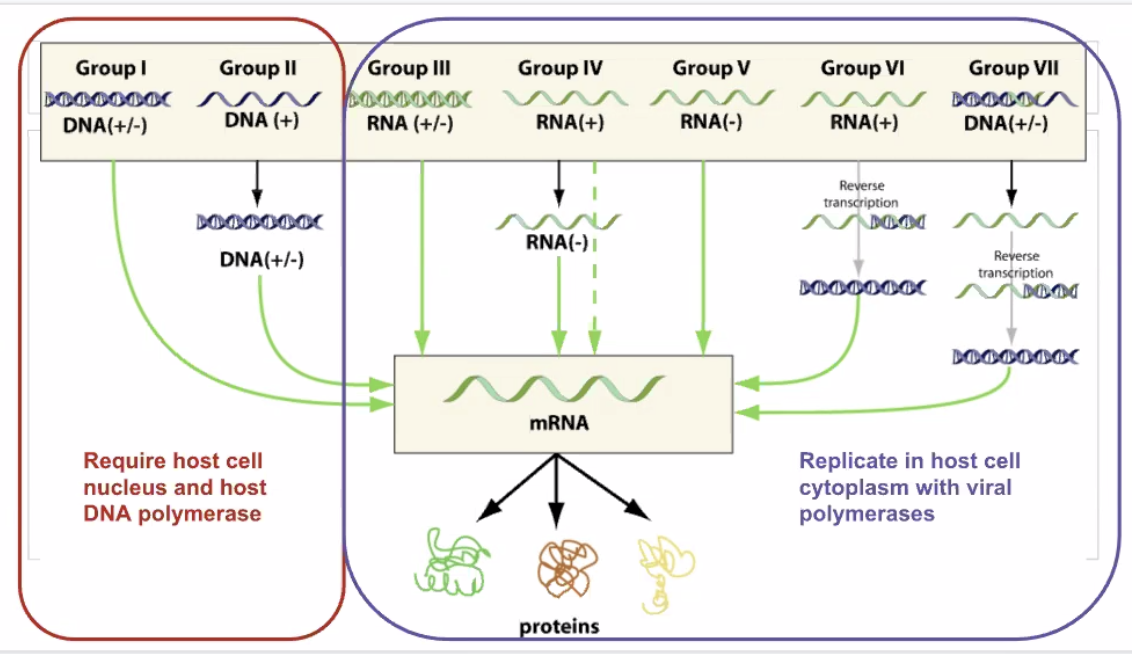
\includegraphics[width=.9\linewidth]{Screen Shot 2020-11-02 at 2.48.22 PM.png}
\caption{Screen Shot 2020-11-02 at 2.48.22 PM.png}
\end{figure}
\end{document}
